
\iffalse
\begin{forest}
  for tree={
    font=\ttfamily,
    grow'=0,
    child anchor=west,
    parent anchor=south,
    anchor=west,
    calign=first,
    inner ysep=0pt,
    edge path={
      \noexpand\path [draw, \forestoption{edge}]
      (!u.south west) +(20pt,0) |- node[fill,inner sep=5pt] {} (.child anchor)\forestoption{edge label};
    },
    before typesetting nodes={
      if n=1
        {insert before={[,phantom]}}
        {}
    },
    fit=band,
    before computing xy={l=40pt}, % Horizontal line length
  }
[
  [\myfolder{NXinstrument}
    [\myfolder{NXsource}]
    [\myfolder{NXdetector}
        [\myfile{counts[100]}]
        [\myfile{gas\_pressure[100]}]
        [\myfile{two\_theta[100]}]
        [\myfolder{NXoff\_geometry}
            [\myfile{vertices[100]}]
            [\myfile{faces[100]}]
        ]
    ]
    [\myfolder{NXmonochromator}]
  ]
  [\myfolder{NXdata}
    [\myfile{counts[100]}]
    [\myfile{two\_theta[100]}]
  ]
  [\myfolder{NXsample}]
]
\end{forest}
\fi

\begin{figure}
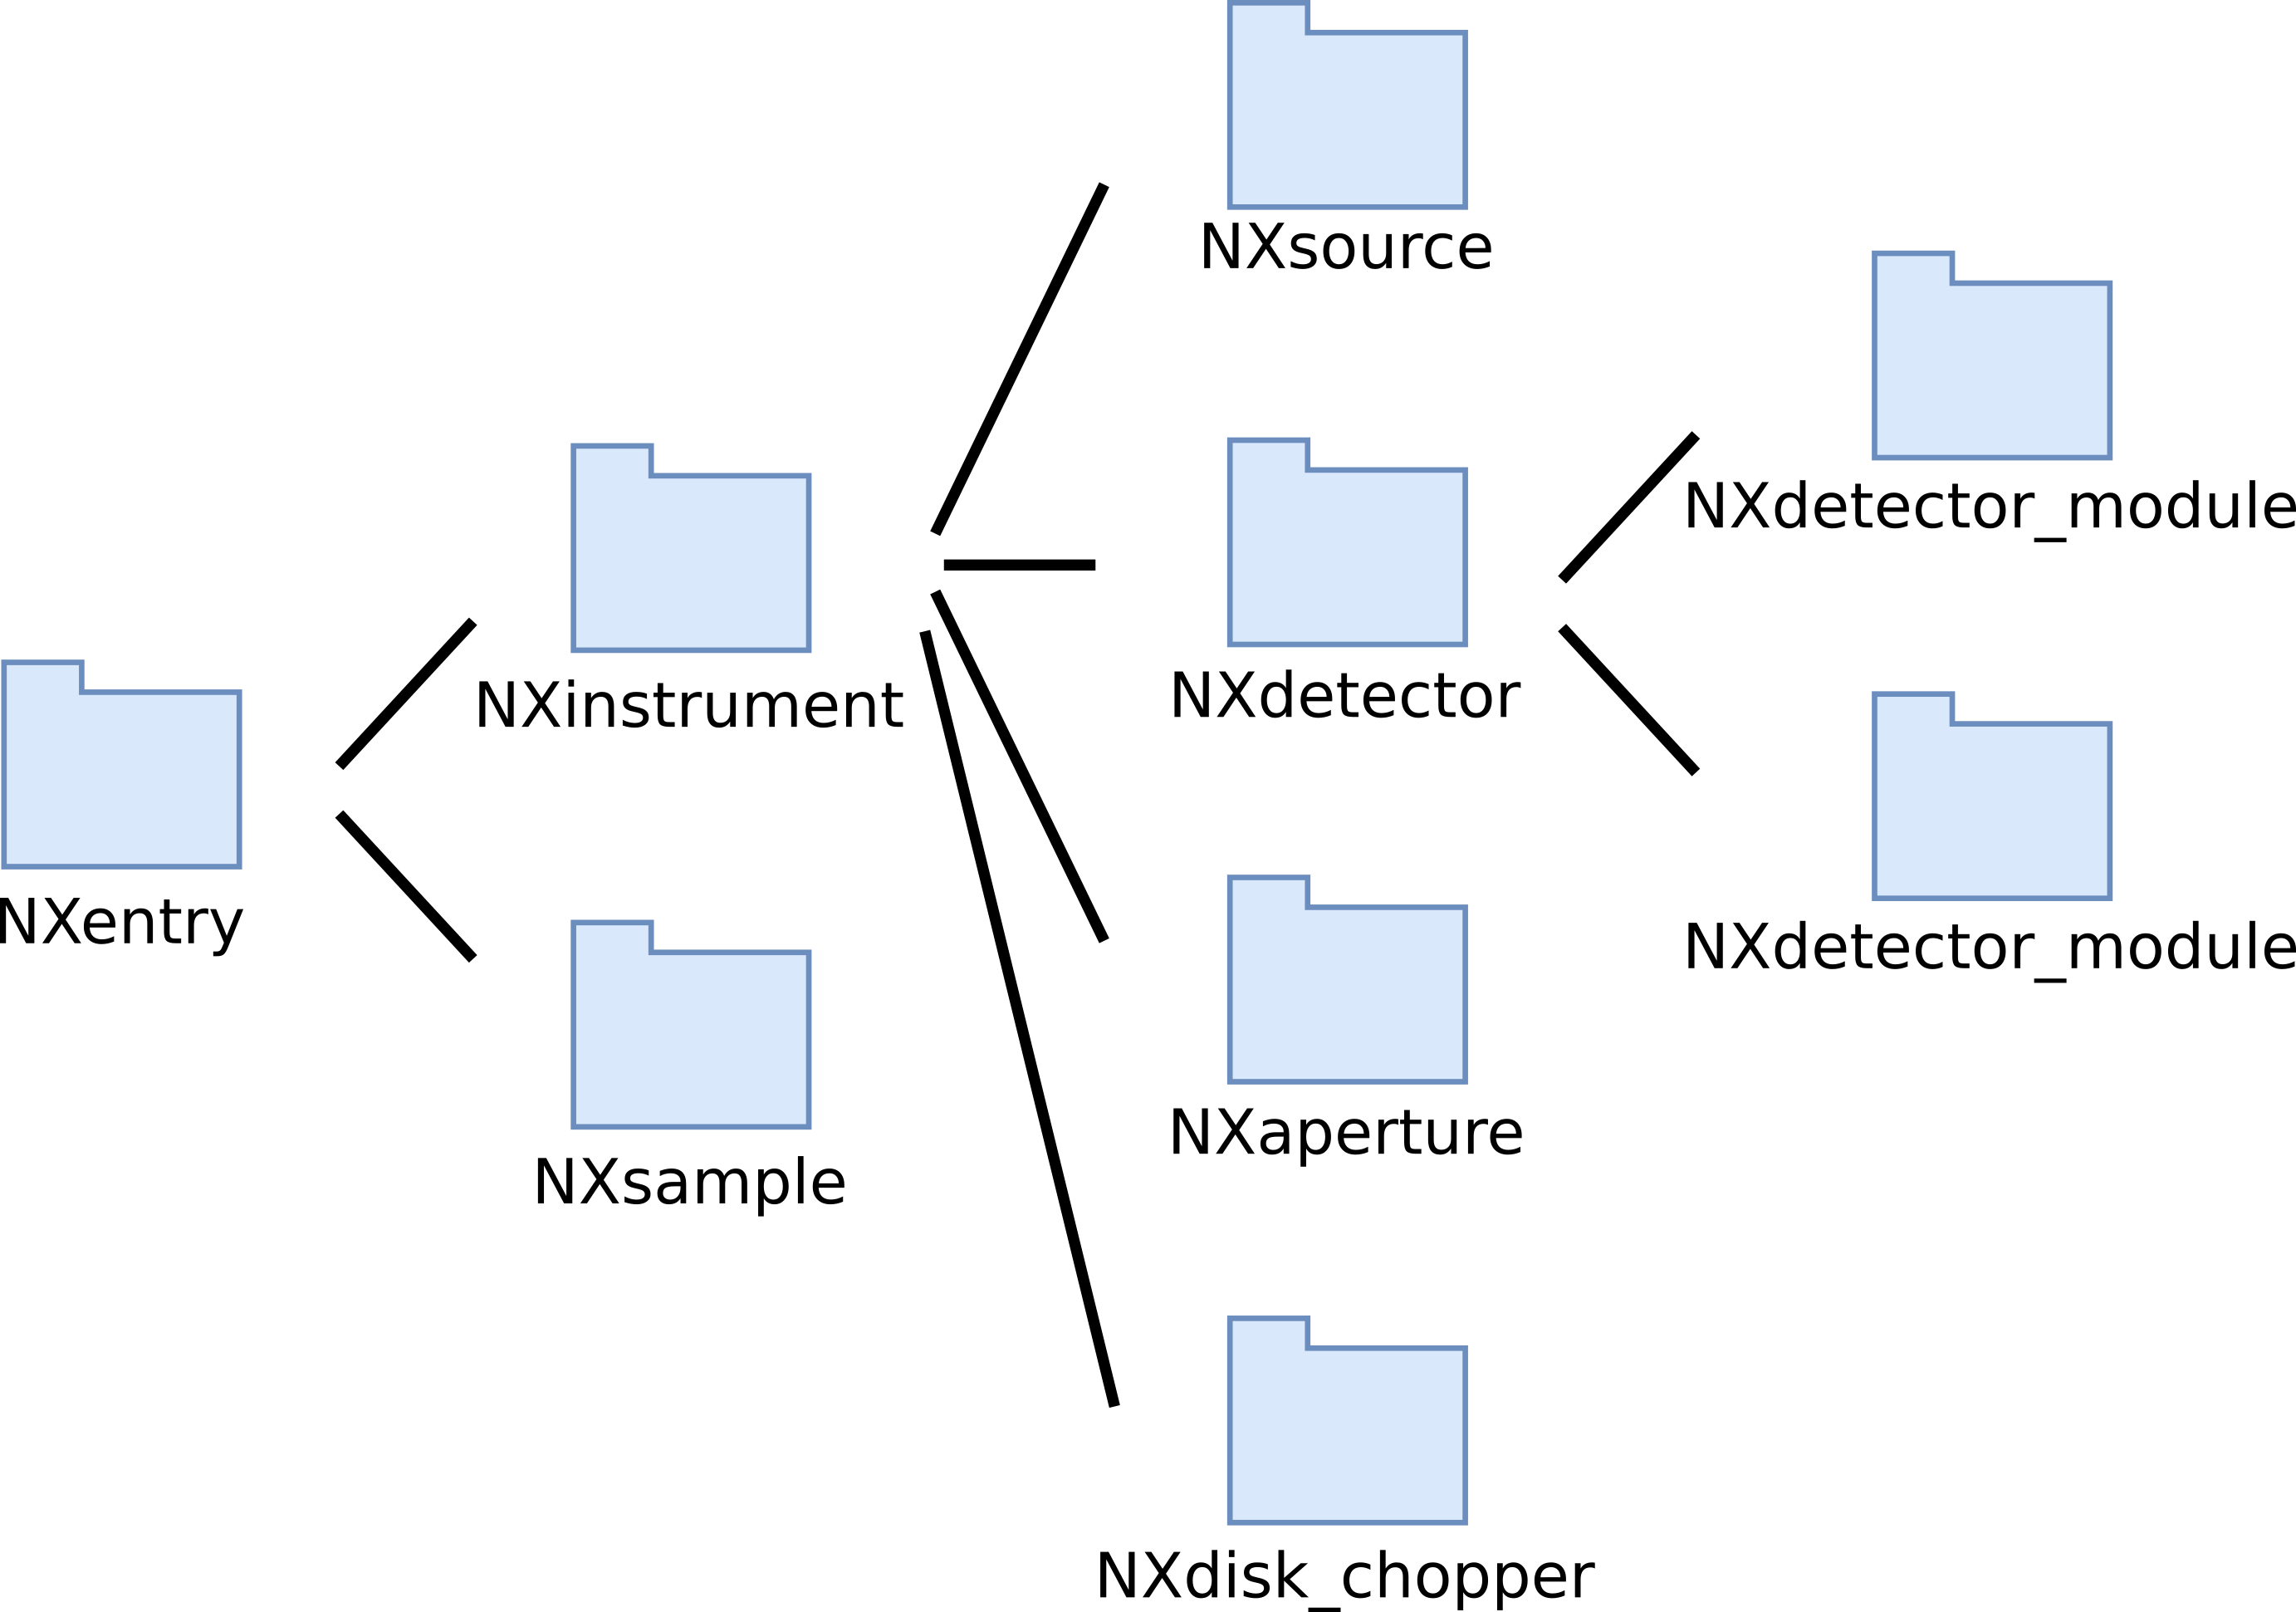
\includegraphics[width=0.6\linewidth]{instrument_arch.png}
\caption{A typical NeXus file layout}
\end{figure}

% What's a shape definition?

The NeXus file format was developed with the aim of:
\begin{itemize}
\item Creating a file format which is common to different neutron facilities.
\item Storing all experiment data in a single file.
\item Allowing experiment data to be loaded into a variety of different software tools without the need for conversion.
\end{itemize}

NeXus is built on top of the HDF5 file format. It adds domain-specific rules for organising data and has a dictionary of well-defined domain-specific file names pertaining to the components used in neutron experiments and their characteristics.
